%%%%%%%%%%%%%%%%%%%%%%%%%%%%%%%%%%%%%%%%%%%%%%%%%%%%%%%%%%
%% BEGIN PREAMBLE
\documentclass[10pt]{article}

%%%% Sets 1 inch margins on document
\usepackage[margin=1in]{geometry}

%%%% For math macros
\usepackage{amsmath}

%%%% Needed for including figures and other images
\usepackage{graphicx}

%%%% Adds ability to adjust document vertical spacing
% usage:
%   \setspace{1.5} % 1.5x for line spacing
\usepackage{setspace}

%%%% Needed for specifying the list items in enumerate env
% eg. (a,b,b) or (i,ii,iii), (1,2,3)
% usage:
%   \begin{enumerate} [label=(\alph*)] % for (a), (b), (c)
\usepackage{enumitem}

%%%% Defines Times New Roman as font
  % for math and text environments
\usepackage{newtxtext,newtxmath}

%%%% For H float option when inserting figure
%   [H] inserts figure _exactly_ where it is typeset
% usage:
%   begin{figure} [H]
\usepackage{float}

%%%% For fancy header and footer ;)
\usepackage{fancyhdr}
\pagestyle{fancy}
\fancyhead[LO,L]{Samuel Barton}
\fancyhead[CO,C]{ENGS31 - Lab 3}
\fancyhead[RO,R]{\today}
\fancyfoot[LO,L]{}
\fancyfoot[CO,C]{\thepage}
\fancyfoot[RO,R]{}
\renewcommand{\headrulewidth}{0.4pt}
\renewcommand{\footrulewidth}{0.4pt}

%%%% Setting margins in tabular environments
% For making equations (esp. fractions) fit in cells vertically
\usepackage{cellspace}
\cellspacetoplimit 4pt
\cellspacebottomlimit 4pt

\usepackage[cachedir=cache]{minted}
\setminted{fontsize=\small,baselinestretch=0.65,linenos}
%% END PREAMBLE %%
%%%%%%%%%%%%%%%%%%%%%%%%%%%%%%%%%%%%%%%%%%%%%%%%%%%%%%%%%%%%%%%

\begin{document}

\setstretch{1.25} % set spacing to 1.25x

% Assignment Name
\begin{centering}
  \section*{LAB 3}
\end{centering}

\subsection*{Deliverable 1: LUT Analysis}

The truth table is the same as last week. It is equivalent to the logic expression: $ O=I_0~I_1~I_2~I_3 $.

\subsection*{Deliverable 2: Counter LUT}

The LUT $ y[0]\_i\_1 $ implements the logic $ O = I_0' $, and the LUT $ y[1]\_i\_1 $ implements the logic $ O = I_0 \oplus I_1 $. These expressions represent the logic for the two least significant bits in a 4-bit counter which we found in homework.

\subsection*{Deliverable 3: Clock Divider Block Diagram}

\begin{figure} [H]
  \center
  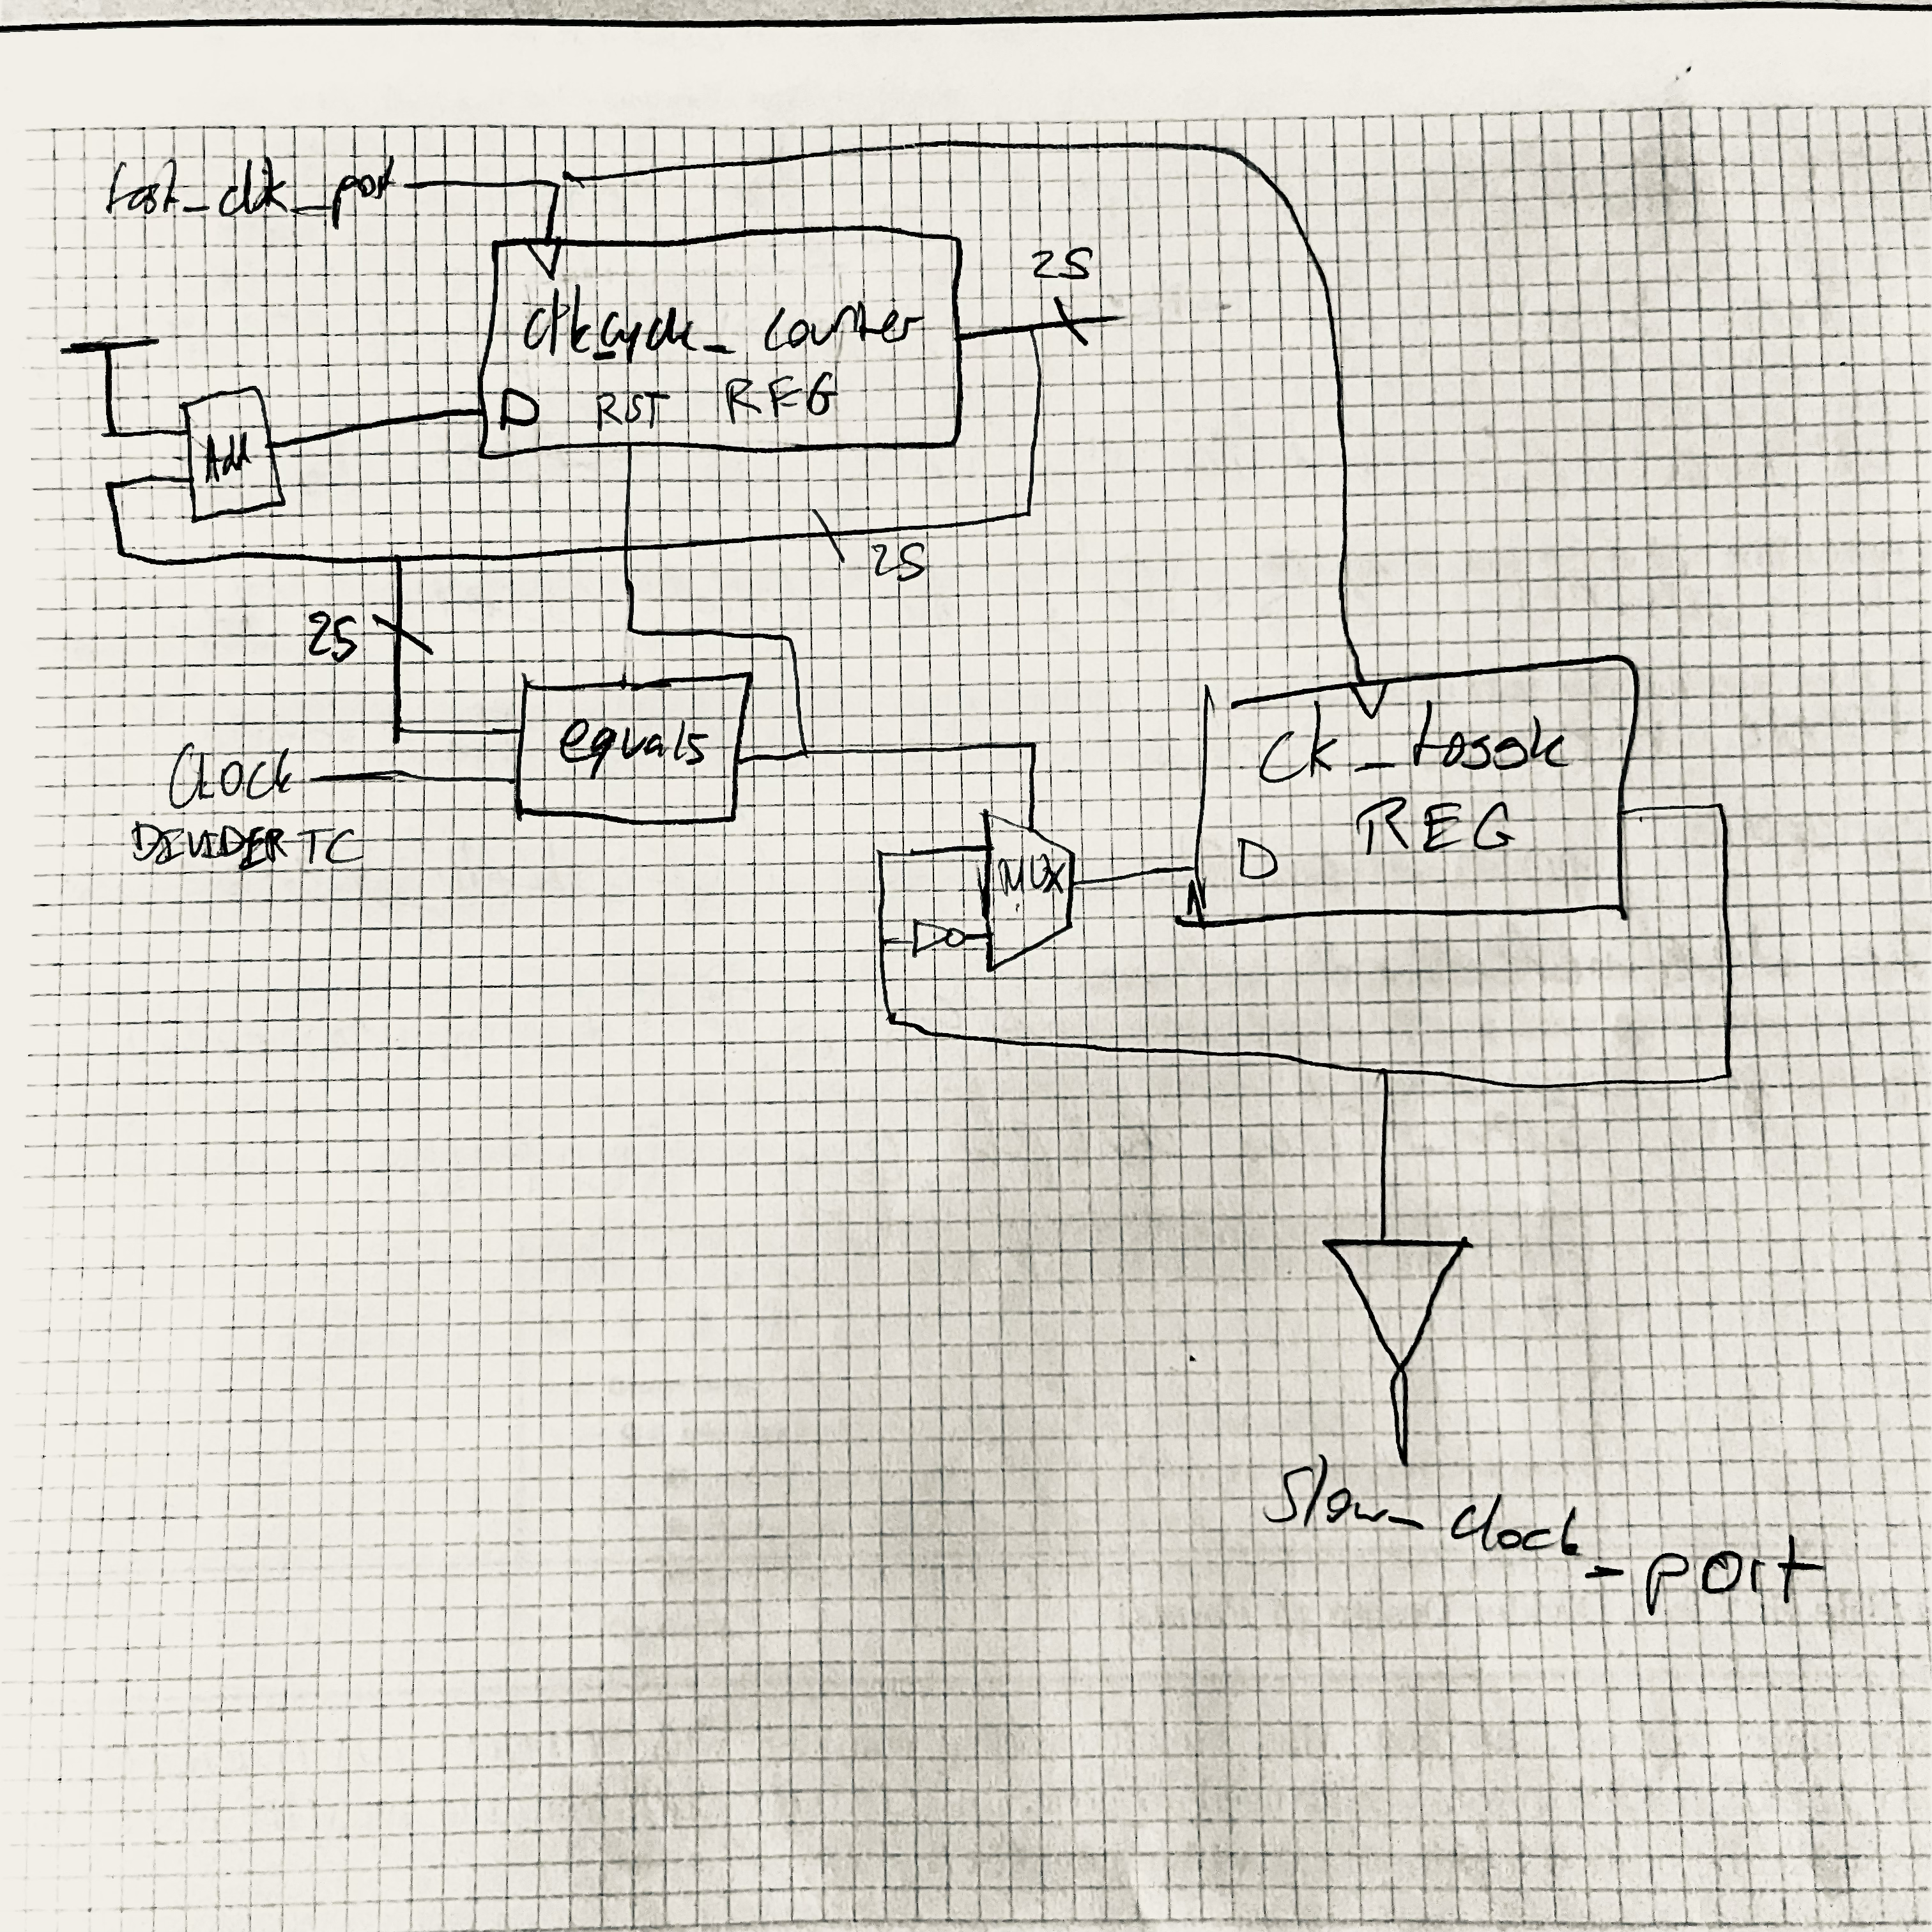
\includegraphics[width=0.9\textwidth]{figures/circuit_drawing.png}
  \caption{Circuit Divider Block Diagram}
\end{figure}

\subsection*{Deliverable 4: Clock Divider Discussion}

The function of this circuit is to convert the fast clock signal (100 MHz) to a slower clock signal (2 Hz).
Using a 25 bit counter, which is needed to store the divisor $ 25 \times 10^{6} $, the circuit resets at this divisor value, and asserts the toggle bit.
The toggle bit corresponds with the slow clock (rising/falling/level) edges as it is connected to the slow\_clock output using BUFD.

\subsection*{Deliverable 5: Clock Divider Design}
\[
  CLOCK\_DIVIDER\_TC := 5
\]

We would need 3 bits for the \texttt{clk\_divider\_counter}.

\subsection*{Deliverable 6: BCD Enumeration}

\begin{figure} [H]
  \center
  \includegraphics[width=0.8\textwidth]{figures/deliverable6_annotated.png}
  \caption{Annotated RTL Schematic for BCD Enumeration}
\end{figure}
 
\subsection*{Deliverable 7: Waveforms}

\begin{figure} [H]
  \center
  \includegraphics[width=0.9\textwidth]{figures/full_sim_annotated.png}
  \caption{Entire Simulation Runtime, Annotated}
\end{figure}

\begin{figure} [H]
  \center
  \includegraphics[width=0.9\textwidth]{figures/rollover_waveform_annoteated.png}
  \caption{Simulation Zoomed-In on Rollover Behavior, Annotated}
\end{figure}

\subsection*{Deliverable 8: Hardware Validation}

\begin{figure} [H]
  \center
  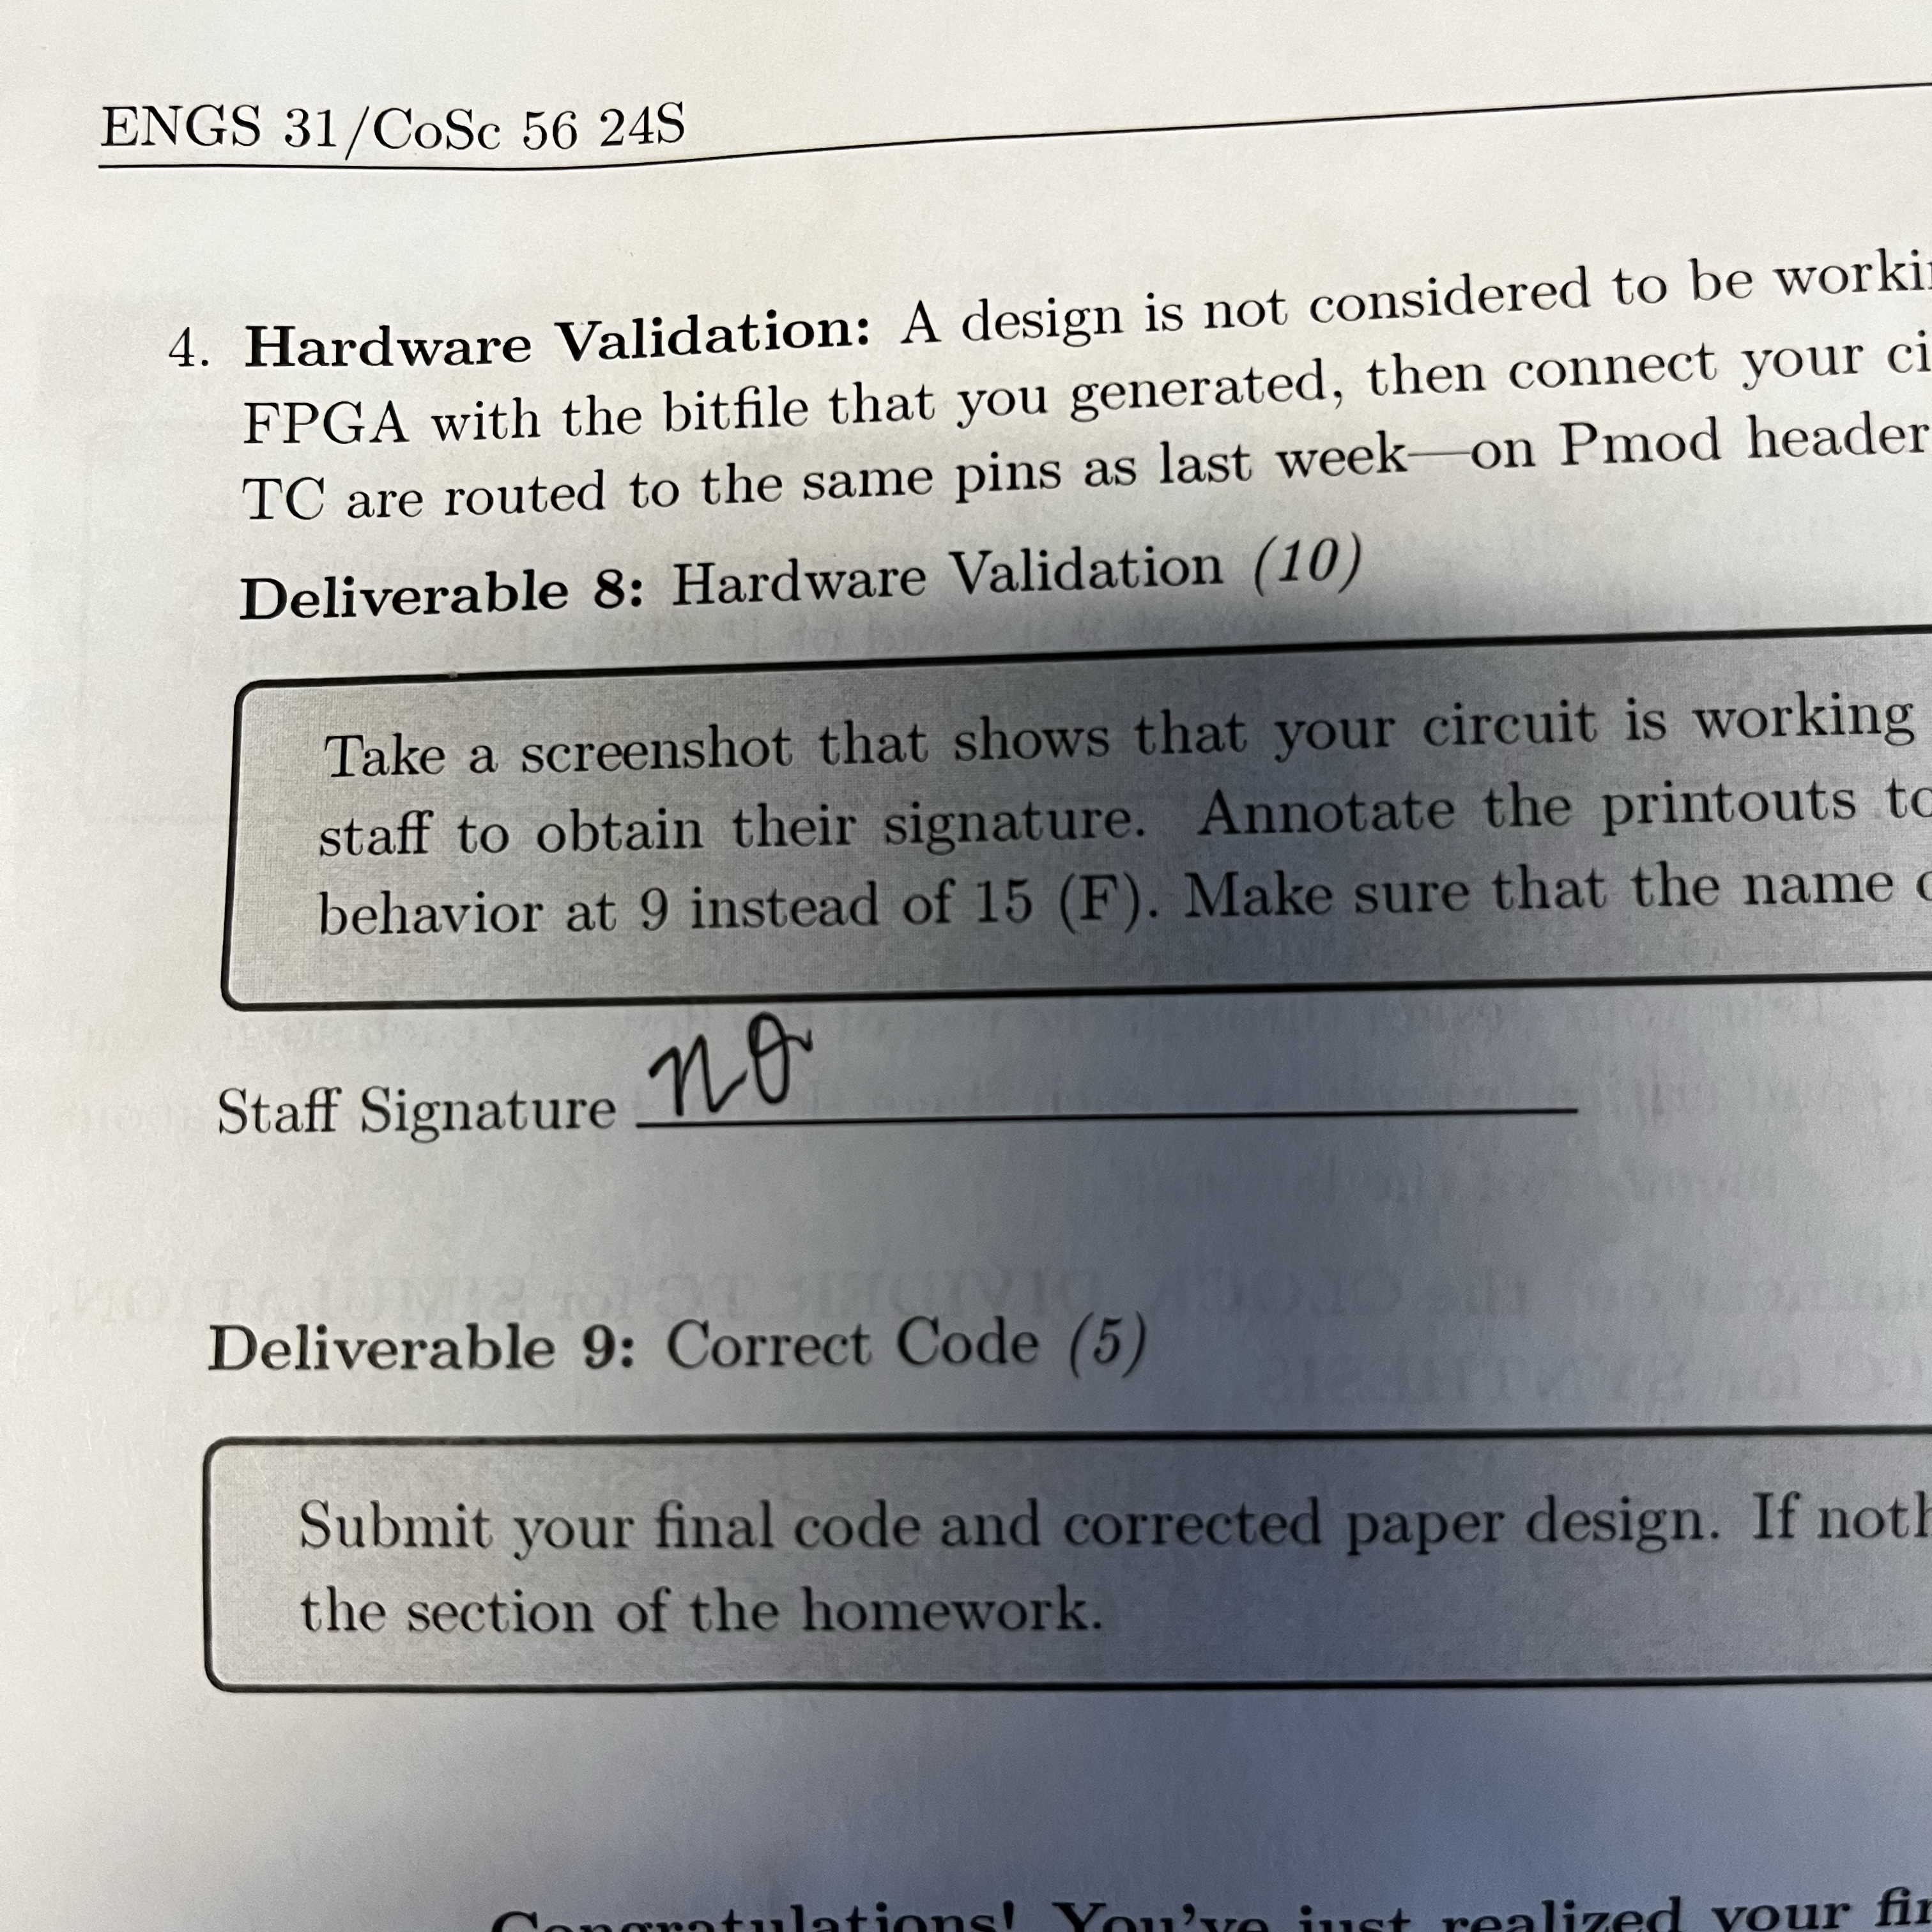
\includegraphics[width=0.4\textwidth]{figures/signature.png}
  \caption{Staff Signature}
\end{figure}

\begin{figure} [H]
  \center
  \includegraphics[width=0.75\textwidth]{figures/normal_operation_annotated.png}
  \caption{Normal Operation of BCD Circuit, Annotated}
\end{figure}

\begin{figure} [H]
  \center
  \includegraphics[width=0.75\textwidth]{figures/reset_multiple_annotated.png}
  \caption{Pressing the Reset Button a Few Times, Annotated}
\end{figure}

\begin{figure} [H]
  \center
  \includegraphics[width=0.75\textwidth]{figures/enable_off_annotated.png}
  \caption{Disabling the Counting, Annotated}
\end{figure}

\subsection*{Deliverable 9: Correct Code}

\begin{figure}[H]
  \inputminted{vhdl}{./vhdl/bcd_digit.vhd}
  \caption{Full VHDL code for \texttt{bcd\_digit.vhd}}
\end{figure}


\end{document}

